\chapter{Przegląd istniejących rozwiązań}
\par
Jako że problem zmiany identyfikatorów plików znany już jest od lat, na rynku istnieje wiele aplikacji próbujących się z nim uporać. Wiele z istniejących rozwiązań zostało zaprojektowanych dla plików konkretnego typulub są modułami większych aplikacji lecz istnieje kilka\footnote{Aplikacje zostały wybrane ze względu na ich popularność i podejście do rozwiązania problemu} implementacji gotowych do ogólnego zastosowania.
\par
Poniżej zostały przedstawione trzy wybrane implementacje wraz z subiektywną opinią o nich.

\section{Bulk Rename Utility}
\begin{figure}[h]
\begin{center}
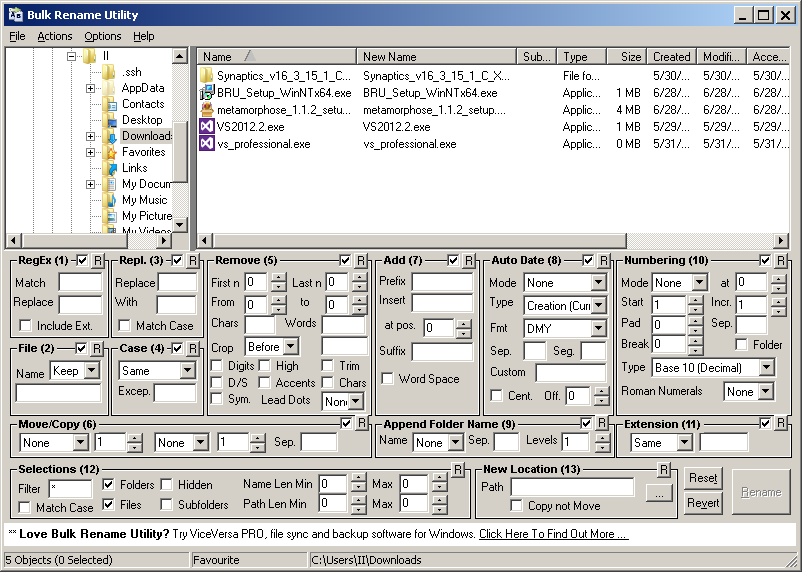
\includegraphics[scale=0.75]{img/bulkrename_window.png}
\end{center}
\caption{Okno główne programu Bulk Rename Utility}
\end{figure}

\par
Jednym z bardziej zaawansowanych i polecanych programów na platformę Microsoft Windows jest \textit{Bulk Rename Utility}. Aplikacja umożliwia ekstrakcje metadanych z plików audio (za pomocą tagów ID3v1) i obrazów zawierających dane EXIF, a także posiada wiele funkcjonalności związanych z modyfikacją istniejącej nazwy --- takich jak wyrażenia regularne.
Wyróżnia się wsparciem dla modyfikacji nazw i atrybutów katalogom, a także zwartym interfejsem .
Program nie wspiera zmiany kolejności wykonywania działań na nazwie --- wszystkie operacje mają swoją pozycje w kolejce wywołania i istnieje jedynie możliwość ich włączenia lub wyłączenia.
\textit{Bulk Rename Utility} posiada również swój odpowiednik --- \textit{Bulk Rename Command} --- który jest oddzielnym programem udostępniającym funkcjonalność programu z linii poleceń.

\section{Métamorphose}
\begin{figure}[h]
\begin{center}
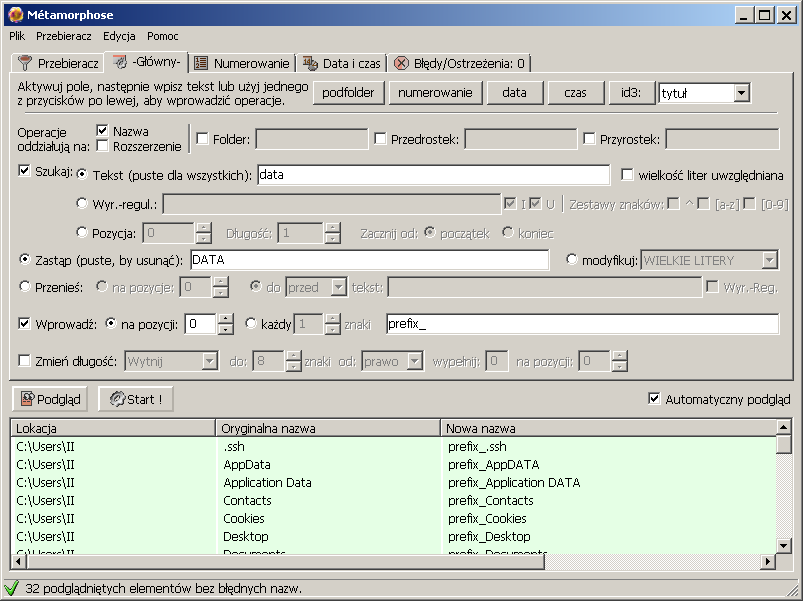
\includegraphics[scale=0.75]{img/metamorphose_window.png}
\end{center}
\caption{Jedna z zakładek programu Métamorphose}
\end{figure}

\par
\textit{Métamorphose} podobnie jak \textit{Bulk Rename Utility} korzysta z wbudowanego zestawu funkcjonalności jednak posiada pewne wsparcie dla szablonów nazw plików. Jest również aplikacją wieloplatformową, a także dzięki zastosowaniu zakładek --- bardziej przejrzystą.

\section{KRename}
\begin{figure}[h]
\begin{center}
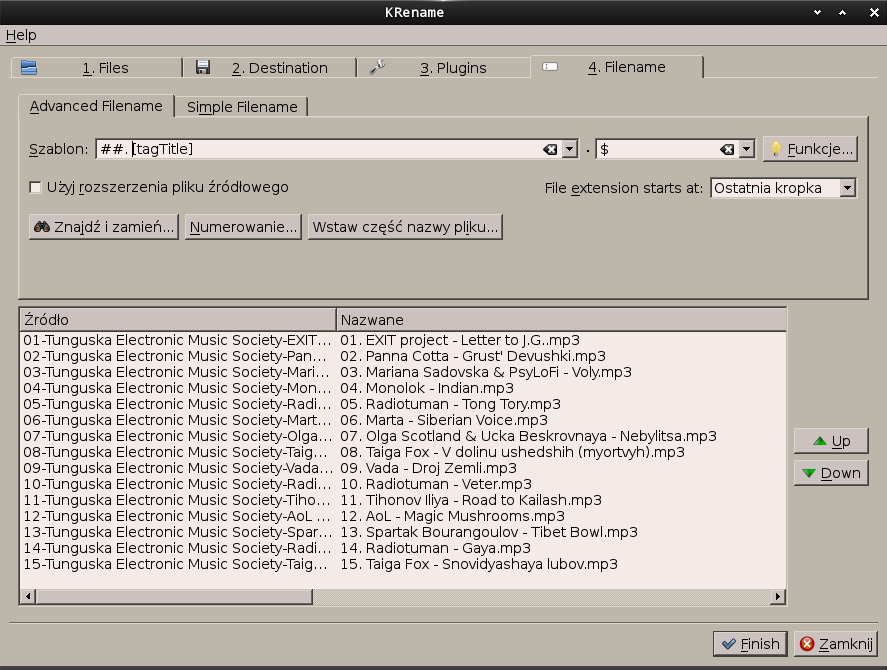
\includegraphics[scale=0.55]{img/krename_window.png}
\end{center}
\caption{Konfiguracja szablonu nazwy pliku w KRename}
\end{figure}

\par
\textit{KRename} w odróżnieniu od poprzednich programów nie posiada wersji dla systemów Windows. Zestaw zakładek pozwala na znalezienie plików, wybranie akcji do wykonania, a także przegląd i edycję wtyczek umożliwiających ekstrakcje danych. Poza trybem edycji szablonu dla nazw plików istnieje prostszy interfejs pozwalający na podstawowe operacje dodania sufiksu lub prefiksu, a także zmianę wielkości znaków w nazwie.\\
Zaletą programu jest duży wybór wtyczek pozwalających także na modyfikacje metadanych samych a nawet zawarcie w nowej nazwie rezultatu wywołania kodu JavaScript.

\section{Inne rozwiązania}
\par
Osoby korzystające z nowoczesnych systemów \texttt{POSIX}-owych posiadają ciekawą alternatywą dla jakichkolwiek specjalizowanych aplikacji --- tekstową powłokę zwaną shellem.\\
Nowoczesne powłoki shell takie jak \texttt{zsh} czy \texttt{bash} posiadają funkcjonalności umożliwiające łączenie wyników wywołań wielu komend co wraz z bogatą liczbą programów dostępnych dla wspomnianych systemów, umożliwia stworzenie polecenia które mogłoby w prosty modyfikować identyfikatory plików.

\begin{lstlisting}[label=shell-rename, caption={Polecenie powłoki zmieniające roszerzenia plików JPEG}]
find ./ -name *.JPG -exec rename -v 's/\.JPG/\.jpg/' {} \;
\end{lstlisting}

\par
Na listingu \ref{shell-rename} zostało pokazane przykładowe polecenie powłoki zamieniające rozszerzenia plików JPEG z '\textit{JPG}' na '\textit{jpg}'.
Wykorzystuje ono trzy programy:
\begin{itemize}
\item \texttt{find} --- znajduje pliki o rozszerzeniu kończącym się na '\textit{.JPG}' (przez zastosowanie parametru \texttt{-name *.JPG})
\end{itemize}
Polecenia realizujące proste zmiany nazw mogą zostać napisane przez średnio-wprawionego użytkownika powłoki jednak bardziej zaawansowane wymagają użycie wielu programów i nie są tak trywialne jak wyżej wymieniony przykład.
